\chapter{GNSS and positioning}
  Global Navigation Satellite Systems (GNSS) are satellite-based systems that provide positioning, 
  navigation, and timing (PNT) services to users worldwide. The most well-known GNSS is the Global 
  Positioning System (GPS).\\
  The use of GPS and other GNSSs has become quite common in several civil application fields, (e.g.,
  transports and personal mobility, agriculture, ICT, ...), so Location Based Services (LBS) are
  becoming more and more important.\\

  In this chapter we will that GNSS users are particularly sensitive to some kinds of attacks, because
  those signals are very weak: for example Replaying broadcast GNSS signals with some delay 
  (meaconing), is enough to trick a user into a wrong position.\\
  \begin{section}{The positioning Problem}
    First of all, we need to define what is a position.\\
    \begin{boxH}
      A position is a set of coordinates, one for each dimension, associated with a reference 
      system.
    \end{boxH}
    \begin{figure}[h]
      \centering
      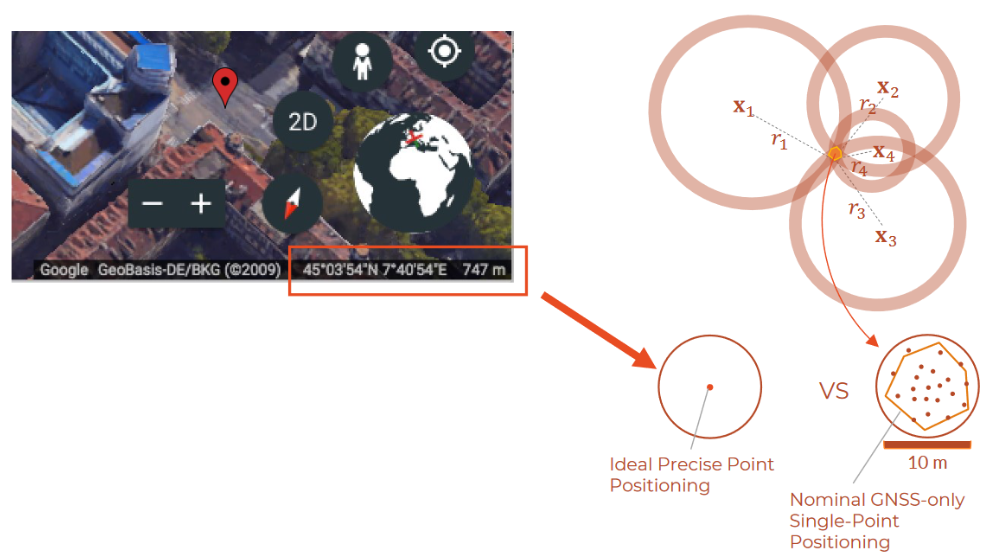
\includegraphics[width=0.8\textwidth]{img/wireless/GNSS position.png}
      \caption{Positioning in a 3D space}
      \label{fig:GNSS position}
    \end{figure}
    As shown in picture \ref{fig:GNSS position}, ideally we would like to have a system that can
    get a precise point positioning over a space, but in reality what we get is a cloud of points
    around the real position, from which the real position is estimated, withing a certain confidence
    interval.\\

    That being said, how is a position estimated?\\
    The information needed to estimate a position is provided by a set of sensors installed on 
    a terminal, such as a smartphone or a GPS receiver.\\
    Some of the most common sensors used are:
    \begin{itemize}
      \item \textbf{Satellite Navigation Chipset}, such as a GPS sensor, which tracks the signals
        from the satellites.
      \item \textbf{Inertial systems}, such as accelerometers and gyroscopes that measure the 
        acceleration and the angular velocity of the terminal.
      \item \textbf{Electronic Compasses}, which provide the orientation of the terminal.
      \item \textbf{Barometers}, which measure the atmospheric pressure.
      \item $\dots$
    \end{itemize}

    Because using all that sensors together to estimate a position is ideal but quite complex,
    a \textbf{data fusion algorithm} is used to combine the information from the sensors and estimate
    the position.\\
    \begin{figure}[h]
      \centering
      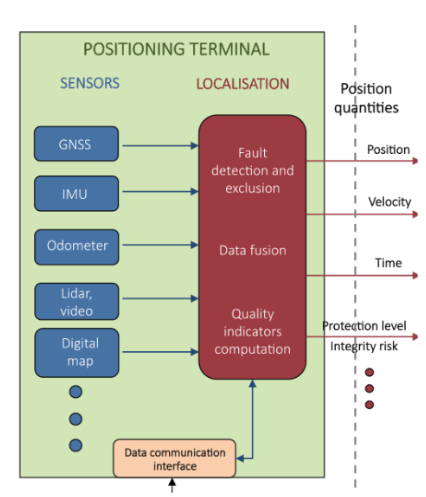
\includegraphics[width=0.3\textwidth]{img/wireless/data fusion algorithms.png}
      \caption{Representation of a data fusion algorithm}
      \label{fig:GNSS data fusion}
    \end{figure}
    In some cases using only the information provides is not enough to estimate a position, so
    some \textit{tricks} are used to improve the accuracy of the position estimation.\\
    For example google maps, when it gets an off road position, uses the information provided and
    maps the position to a point between some landmarks positioned on the road, as shown in picture
    \ref{fig:maps example}.\\

    \begin{figure}[h]
      \centering
      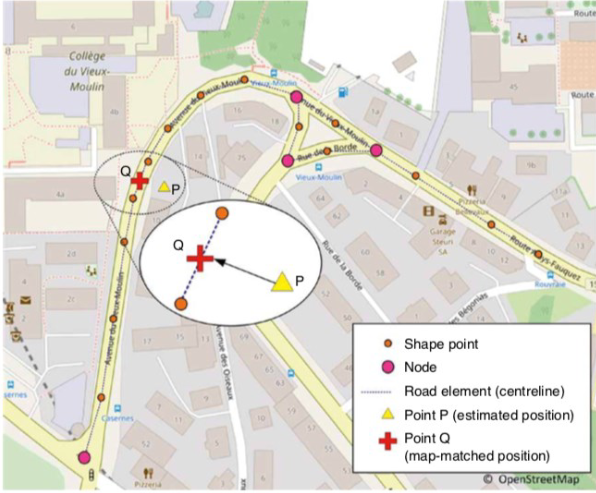
\includegraphics[width=0.6\textwidth]{img/wireless/maps example.png}
      \caption{Example of position estimation using landmarks}
      \label{fig:maps example}
    \end{figure}
  \end{section}

  \begin{section}{Satellite Navigation Systems and Segments}
    A little of history: the first satellite navigation system was put in space by the US Department
    of Defense in 1978. But it was only in the early 2000s that the system was opened to civil users.\\
    The european counterpart of the GPS is the Galileo system, which was put in space in 2017.\\
    \begin{figure}[h]
      \centering
      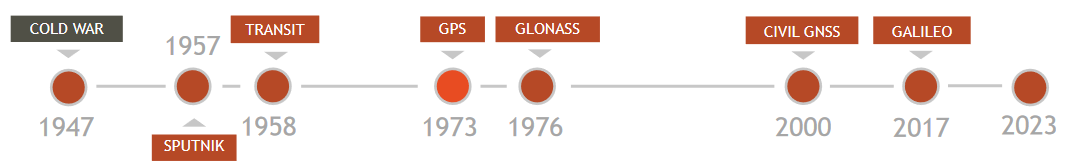
\includegraphics[width=0.9\textwidth]{img/wireless/GNSS history.png}
      \caption{History of GNSS systems}
      \label{fig:GNSS systems history}
    \end{figure}
    To provide a global coverage, a GNSS system is composed of a constellation of satellites, which
    are positioned in such a way that at least 4 satellites are visible from any point on the Earth.\\

    There are 4 main GNSS systems nowadays:
    \begin{itemize}
      \item \textbf{GPS} (USA)
      \item \textbf{Galileo} (Europe)
      \item \textbf{GLONASS} (Russia)
      \item \textbf{Beidou} (China)
    \end{itemize}
    which orbits at different altitudes and inclinations.\\
    Each of those systems  continuously transmit navigation signals in different frequencies in $L$ 
    band, as shown in picture \ref{fig:GNSS band}.\\

    \begin{figure}[h]
      \centering
      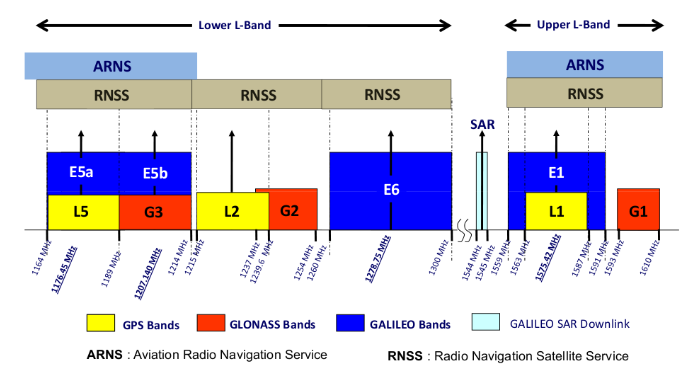
\includegraphics[width=0.8\textwidth]{img/wireless/GNSS band.png}
      \caption{Division of the $L$ band for GNSS systems}
      \label{fig:GNSS band}
    \end{figure}

    All those system are composed of 3 main segments:
    \begin{itemize}
      \item \textbf{Space Segment}, which is composed of the satellites, which continuously transmit
        the signals.
      \item \textbf{Control Segment}, which is composed of the ground stations that monitor the 
        satellites and send them the corrections.
      \item \textbf{User Segment}, which is composed of the users that receive the signals from the
        satellites and estimate their position. It performs 3 core functions:
        \subitem - Identification of the satellites in view
        \subitem - Measurement of the user-satellite distance
        \subitem - Run a PVT(Position, Velocity, Time) estimation algorithm
    \end{itemize}
    \begin{figure}[h]
      \centering
      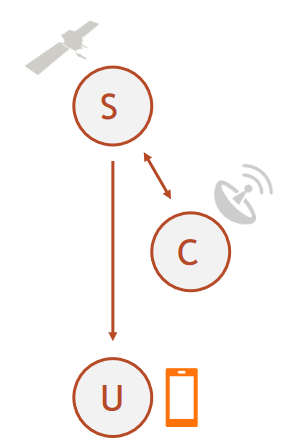
\includegraphics[width=0.2\textwidth]{img/wireless/GNSS segments.png}
      \caption{Schema of the GNSS segments}
      \label{fig:GNSS segments}
    \end{figure}
    \begin{subsection}{GNSS signals}
      The GNSS satellites continuously transmit navigation signals in different frequencies in $L$ 
      band.\\
      Those signals are made up of different components, as shown in picture \ref{fig:GNSS signals}.\\
      The carrier modulate the data at the right frequency, the spreading code to perform multiple
      access, allowing to distinguish information from different satellites and demultiplexing the
      signals from the same satellite, , and the navigation data that contains the information 
      about the satellite position and the time.\\

      The navigation data allow the user to compute the travelling time from the satellite to the receiver,
      and the satellite position at any time.\\
      Using both the satellite position and the travelling time, the user can estimate its position
      , velocity and time(PVT).\\

      \begin{figure}[h]
        \centering
        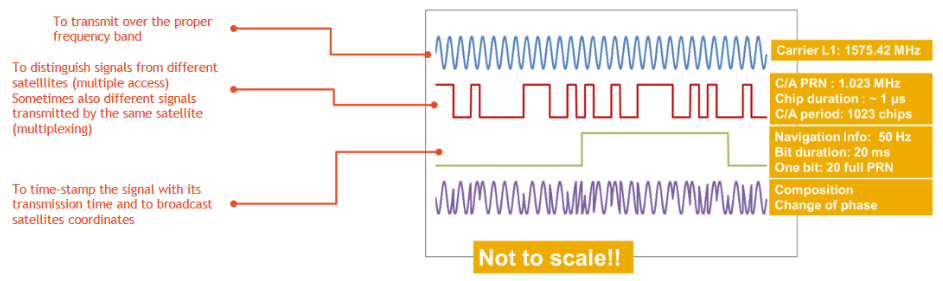
\includegraphics[width=0.8\textwidth]{img/wireless/GNSS signal scheme.png}
        \caption{Scheme of the signals that make up the GNSS signal}
        \label{fig:GNSS signals}
      \end{figure}
    \end{subsection}

  \end{section}
  \begin{section}{Multilateration}
    Lets take a look at figure \ref{fig:GNSS multilateration problem}.\\
    We have a satellite that sends a signal $R_i$ to a user $x$, which would like to estimate 
    three coordinates $\langle x, y, z \rangle$.\\
    The signal contains the position of the satellite and the departure time of the message
    $T_{TX}$.\\
    The receiver measures the arrival time of the signal $T_{RX}$, and computes the distance
    between the receiver and the satellite $R_i$ as follows:
    \begin{equation}
      R_i = c\cdot \tau = c(T_{RX} - T_{TX})
      \label{eq:GNSS distance}
    \end{equation}
    where $c$ is the speed of light, which is the propagation speed of the signal, and $\tau$ is the
    \textit{time of flight} of the signal.\\
    In other words, the distance is the traveling time of the signal multiplied by propagation time
    in the free space.\\

    \begin{figure}[h]
      \centering
      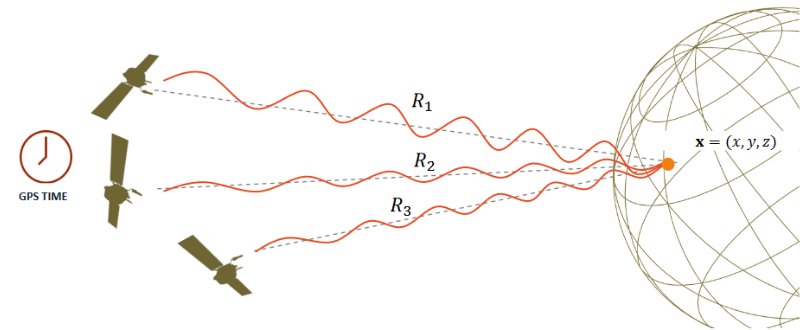
\includegraphics[width=0.8\textwidth]{img/wireless/GNSS multilateration problem.png}
      \caption{Multilateration problem}
      \label{fig:GNSS multilateration problem}
    \end{figure}

    One measurement is not enough to estimate the position of the receiver, so at least 3 measurements
    are needed.\\
    \begin{boxH}
      We call this procedure \textbf{multilateration}, or the process of determining the position of an object
      by measuring the time of arrival of the signals from multiple sources.
    \end{boxH}

    But knowing the distance only tells us that the receiver is on a sphere centered on the satellite
    with radius $R_i$. It can be at any point on the sphere.\\
    If we have 2 satellites, we have 2 spheres, and the receiver is at the intersection of the two
    spheres.\\
    If we have 3 satellites, we have 3 spheres, and the receiver is at the intersection of the 3
    spheres.\\
    Unfortunately things are never that simple, but it gives the rough idea of how multilateration
    works.\\

    \begin{figure}[h]
      \centering
      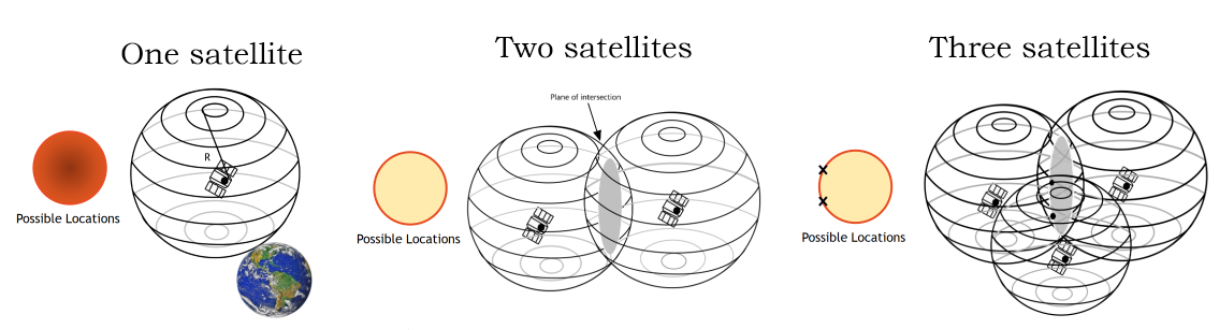
\includegraphics[width=\textwidth]{img/wireless/multilateration comparison.png}
      \caption{Multilateration with 1, 2 and 3 satellites}
      \label{fig:Multilateration comparison}
    \end{figure}
  \end{section}
  \begin{section}{GNSS Functional basics}
    Lets add more detail to multilateration.\\
    If a satellite trasmit a pulse at time $t_0$, the receiver will receive it at time $t_0+\tau$,
    where $\tau$ is the time it takes for the signal to travel from the satellite to the receiver.\\
    We already saw in equation \ref{eq:GNSS distance} that the distance between the satellite and the
    receiver is equal to the time of flight of the signal multiplied by the speed of light.\\

    To get the distance, we only need to timestamp correctly the time of arrival of the signal.
    Yet, calculating the time of flight is not that simple, because the satellite and the receiver
    must be \textbf{synchronized} to allow the transmission time and the reception time to be on the 
    same time scale, and to be precise. Otherwise the distance estimation would be very off: 
    a signal that travels at the speed of light for 1 second travels 300000 km.\\
    In fact, the satellite host an \textbf{atomic clock}, which is a very precise clock that allows
    the satellite to timestamp the signal with a very high precision. They are also synchronized thanks
    to the control segment.\\
    The receiver also has a clock, but it is most likely not as precise as the atomic clock. 
    For this reason, the bias of the user torward the GNSS time scale $\delta t_u$ is unknown.\\
    The measured distance is then different from the geometric range and it is referred
    to as \textbf{pseudorange}, which is defined as:
    \begin{equation}
      \rho = c \cdot \tau + c \cdot \delta t_u
      \label{eq:GNSS pseudorange}
    \end{equation}

    There's also the bias of the satellite toward the scale $\delta t_u$. 
    This value is usually small and stable over time. The ground segment computes a bias $\delta t^S$
    that is uploaded to the satellite, and that the receiver can use to compute the right time of 
    flight.\\
    For those reason, we consider it to be zero, because it can be corrected.\\

    On the other hand, $\delta t_u$ cannot, the only thing we can do is keep it, so the position 
    is estimated by measuring the different pseudoranges from 4 different satellites, the minimum
    number of satellites in Line of Sight to estimate the position.\\
    This is because 3 satellites are needed to estimate the coordinates of a position, and the fourth
    satellite is needed to estimate the bias $\delta t_u$.\\
    If a larger number of satellites is in view a better estimation is possible.\\

    \begin{figure}[h]
      \centering
      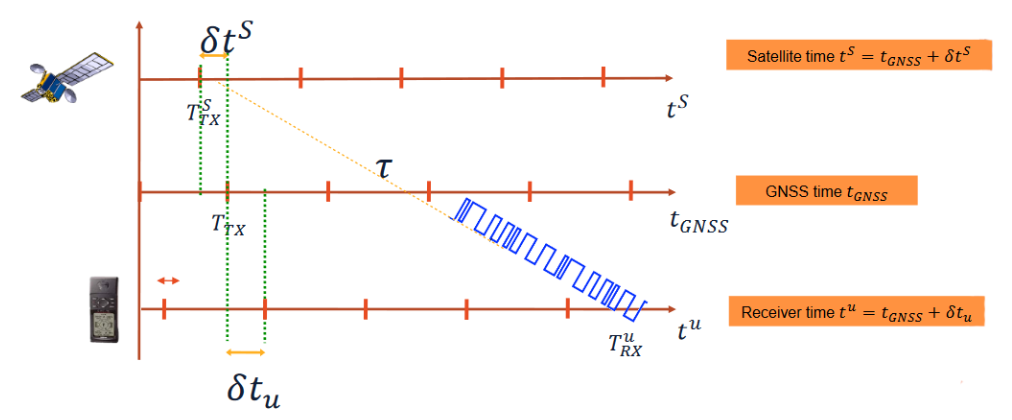
\includegraphics[width=0.8\textwidth]{img/wireless/GNSS bias.png}
      \caption{Graphical representation of the bias $\delta t_u$ on the GNSS timescale}
      \label{fig:GNSS pseudorange}
    \end{figure}

    To sum it up, in GNSSs the user position is obtained through:
    \begin{itemize}
      \item \textbf{satellites} that broadcast that transmits timestamps.
      \item \textbf{Pseudoranges}, estimated trough one-way-arrival measurements
        receiver, plus the bias of the user toward the GNSS time scale.
      \item \textbf{Multilateration} based on the measurements
    \end{itemize}

    \begin{subsection}{The estimation problem}
      We have the measurements, but we need to estimate the position of the receiver.\\
      The relationship between the pseudoranges can be written as:
      \begin{equation}
        \begin{cases}
          \rho_1 = \sqrt{(x_1 - x_u)^2 + (y_1 - y_u)^2 + (z_1 - z_u)^2} + c\delta t_u\\
          \rho_2 = \sqrt{(x_2 - x_u)^2 + (y_2 - y_u)^2 + (z_2 - z_u)^2} + c\delta t_u\\
          \rho_3 = \sqrt{(x_3 - x_u)^2 + (y_3 - y_u)^2 + (z_3 - z_u)^2} + c\delta t_u\\
          \rho_4 = \sqrt{(x_4 - x_u)^2 + (y_4 - y_u)^2 + (z_4 - z_u)^2} + c\delta t_u\\
        \end{cases}
        \label{eq:GNSS pseudorange relationship}
      \end{equation}
      where $\langle x_i, y_i, z_i \rangle$ are the coordinates of the satellites(which are known),
      and $\langle x_u, y_u, z_u \rangle$ are the coordinates of the user(which are unknown as the bias).

      The goal is to invert the relationship and find the user coordinates and the bias given the
      pseudoranges.\\
      It is a non-linear estimation problem which is linearized through Taylor expansion 
      And solved through Least Mean Square Solutions or Bayesian Filters (e.g. Kalman).\\

      The generic pseudorange, which is a nonlinear relationship,
      \begin{equation*}
        \rho_i = \sqrt{(x_i - x_u)^2 + (y_i - y_u)^2 + (z_i - z_u)^2} + c\delta t_u
      \end{equation*}
      can be approximated through the Taylor expansion around a known location used as a linearization point
      (a point that is close to the real solution) $\langle \hat{x}_u, \hat{y}_u, \hat{z}_u, \hat{\delta t}_u \rangle$:
      \begin{equation*}
        \hat{\rho}_i = \sqrt{(x_i - \hat{x}_u)^2 + (y_i - \hat{y}_u)^2 + (z_i - \hat{z}_u)^2} + c\hat{\delta t}_u
        \label{eq:GNSS linearization}
      \end{equation*}
      To put it into a graphical prospective, take a look at figure \ref{fig:GNSS linearization}.\\
      If we choose a linearization point, we need to know the difference $\Delta x_u$ between the real
      position and the linearization point. If we can estimate it, which is easier because it is a 
      linear problem, we can estimate the user position.\\


      \begin{figure}[h]
        \centering
        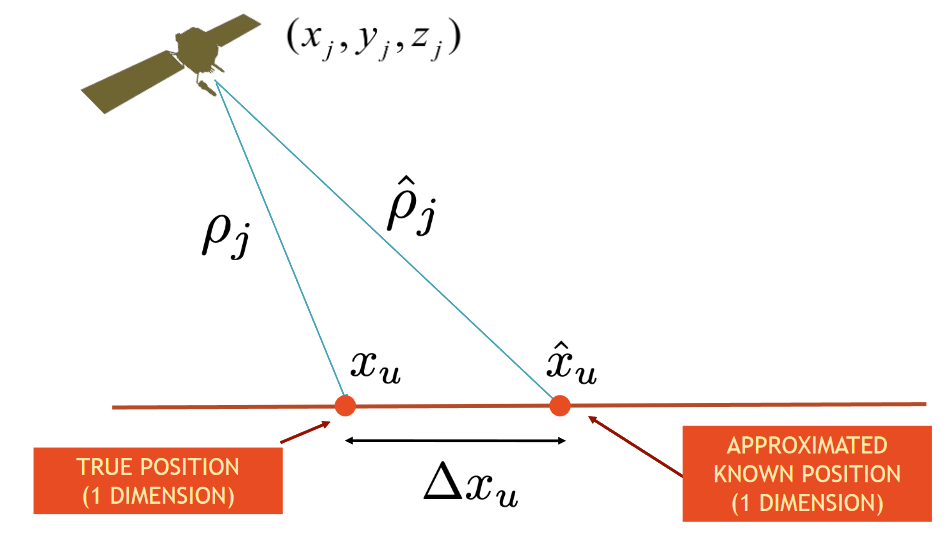
\includegraphics[width=0.5\textwidth]{img/wireless/linearization scenario.png}
        \caption{Graphical representation of the linearization of the pseudorange in one dimension}
        \label{fig:GNSS linearization}
      \end{figure}
      We can expand this concept to the general formula \ref{eq:GNSS linearization} as the difference 
      between the real position and the linearization point:
      \begin{equation}
        \begin{cases}
          \Delta x_u = x_u - \hat{x}_u\\
          \Delta y_u = y_u - \hat{y}_u\\
          \Delta z_u = z_u - \hat{z}_u\\
          \Delta \delta t_u = \delta t_u - \hat{\delta t}_u\\
        \end{cases}
        \label{eq:GNSS linearization difference}
      \end{equation}
      The linearized pseudorange can be written as:
      \begin{equation}
        \delta \rho_j = \hat{\rho}_j - \rho_j = a_{xj}\Delta x_u + a_{yj}\Delta y_u + a_{zj}\Delta z_u + a_{tj}\Delta \delta t_u
        \label{eq:GNSS linearized pseudorange}
      \end{equation}
      The coefficients $a_{ij}$ are the partial derivatives of the pseudorange with respect to the
      user position and the bias, obtained through the Taylor expansion.\\
      They can be written as:
      \begin{equation}
        \begin{cases}
          a_{xj} = \frac{x_j - \hat{x}_u}{\hat{\rho}_j}\\
          a_{yj} = \frac{y_j - \hat{y}_u}{\hat{\rho}_j}\\
          a_{zj} = \frac{z_j - \hat{z}_u}{\hat{\rho}_j}\\
          a_{tj} = \frac{c}{\hat{\rho}_j}
        \end{cases}
        \label{eq:GNSS linearized coefficients}
      \end{equation}
      where 
      \begin{equation*}
        \hat{\rho}_j = \sqrt{(x_j - \hat{x}_u)^2 + (y_j - \hat{y}_u)^2 + (z_j - \hat{z}_u)^2} + c\hat{\delta t}_u
      \end{equation*}
      that being the geometrical distance between the linearization point and the satellite.\\
      This allows us to write our relationship as:
      \begin{equation}
        \begin{cases}
          \delta \rho_1 = a_{x1}\Delta x_u + a_{y1}\Delta y_u + a_{z1}\Delta z_u + a_{t1}\Delta \delta t_u\\
          \delta \rho_2 = a_{x2}\Delta x_u + a_{y2}\Delta y_u + a_{z2}\Delta z_u + a_{t2}\Delta \delta t_u\\
          \delta \rho_3 = a_{x3}\Delta x_u + a_{y3}\Delta y_u + a_{z3}\Delta z_u + a_{t3}\Delta \delta t_u\\
          \delta \rho_4 = a_{x4}\Delta x_u + a_{y4}\Delta y_u + a_{z4}\Delta z_u + a_{t4}\Delta \delta t_u\\
        \end{cases}
        \end{equation}
        that can be also rewrited in a matrix form as:
        \begin{equation}
        \begin{bmatrix}
          \delta \rho_1\\
          \delta \rho_2\\
          \delta \rho_3\\
          \delta \rho_4\\
        \end{bmatrix}
        =
        \begin{bmatrix}
          a_{x1} & a_{y1} & a_{z1} & a_{t1}\\
          a_{x2} & a_{y2} & a_{z2} & a_{t2}\\
          a_{x3} & a_{y3} & a_{z3} & a_{t3}\\
          a_{x4} & a_{y4} & a_{z4} & a_{t4}\\
        \end{bmatrix}
        \begin{bmatrix}
          \Delta x_u\\
          \Delta y_u\\
          \Delta z_u\\
          \Delta \delta t_u\\
        \end{bmatrix}
        \label{eq:GNSS linearized matrix}
      \end{equation}
      where $a_{tj}$ can be approximated as $1$ because the bias is usually small.\\
      This matrix representation is easier to invert, in fact 
      \begin{equation*}
        \delta x= H^{-1}\delta \rho
      \end{equation*}
      which is our solution: the user position.\\
      \begin{subsubsection}{The Least Squares Solution}
        The method above can only be used if the number of satellites is small(4 or less), because 
        otherwise the matrix $H$ would be non-square and non-invertible.\\
        If the number of satellites is larger, it is possible to use the Least Squares Solution.\\
        The solution would be 
        \begin{equation}
          \Delta x = (H^TH)^{-1}H^T\delta \rho
          \label{eq:GNSS least squares}
        \end{equation}
        where $H^T$ is the transpose of the matrix $H$.\\
      \end{subsubsection}
      \end{subsection}

    \begin{section}{Positioning Errors}
      We know that that channel is unpredictable, so the pseudorange is most likely affected by errors,
      due to things such as noise and propagation.\\
      We can redifine our pseudorange model as:
      \begin{equation}
        \rho_i = \sqrt{(x_i - x_u)^2 + (y_i - y_u)^2 + (z_i - z_u)^2} + b_{ut} + \epsilon
        \label{eq:GNSS pseudorange error}
      \end{equation}
      where $b_{ut}$ is the bias of the user toward the GNSS time scale, and $\epsilon$ is the error.\\

      We also need to modify the solution accordingly:
      \begin{equation}
        \Delta x = [(H^TH)^{-1}H^T]\delta \rho
        \label{eq:GNSS least squares error}
      \end{equation}
      where $\delta \rho$ is the error in the pseudoranges.\\
      Basically, we have a portion of the formula that depends on the geometry of the satellites(
      $(H^TH)^{-1}H^T$) and a portion that depends on the errors in the pseudoranges which is
      upredictable.\\
      As it is possible to observe, the position of the satellite influence the error in the pseudorange,
      fore example amplifying it.\\
      
      The causes of the errors in the pseudorange are shown in figure \ref{fig:GNSS errors}.\\
      The relativistic effect on the clock, the fact that even if the clocks are synchronized, they
      move at different speeds, can be corrected because it is predictable.\\
      The atmoshpere too influences the signal, but it can be corrected because it is predictable.\\
      Some of them cannot be corrected, such as the multipath effect, the fact that the signal can
      bounce off buildings and arrive at the receiver later than expected.\\

      \begin{figure}[h]
        \centering
        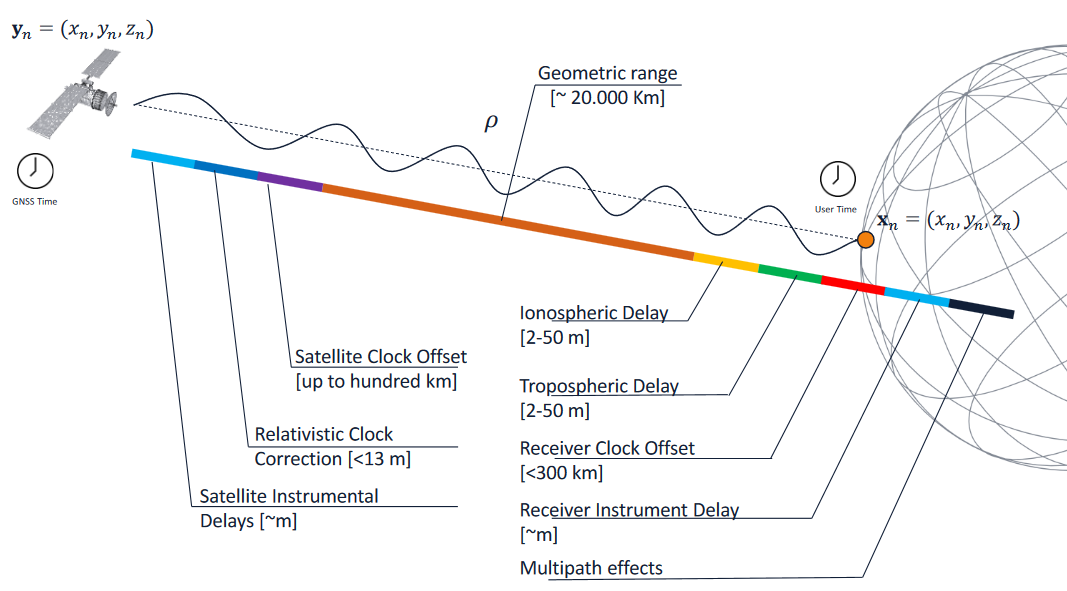
\includegraphics[width=0.8\textwidth]{img/wireless/GNSS errors.png}
        \caption{Causes of the errors in the pseudorange}
        \label{fig:GNSS errors}
      \end{figure}

      \begin{subsection}{User Equivalent Range Error}
        The summary of the total error budget affecting a pseudorange from the user's point of view 
        is called the \textbf{user equivalent range error} (UERE).\\
        Thus, we can model the pseudorange error as a random variable with a mean of $0$ and a standard
        deviation of $\sigma_{\text{UERE}}$.\\
        After correcting known sistematic errors, the unknown ones can be modelled as a Gaussian 
        distribution, with a mean of $0$ and a variance $\sigma_{\text{UERE}}^2$, obtained as the sum
        of other residual contributions:
        \begin{equation}
          \sigma_{\text{UERE}} = \sqrt{\sum_{j} \sigma^2_j [m]}
        \label{eq:GNSS UERE}
      \end{equation}
      \end{subsection}

      \begin{subsection}{The Geometrical Factor}
        Errors makes the solution more uncertain, but its not the only factor that influences the
        accuracy of the solution.\\
        The geometrical distribution of satellites affects the precision of estimated position too

        \begin{figure}[h]
          \centering
          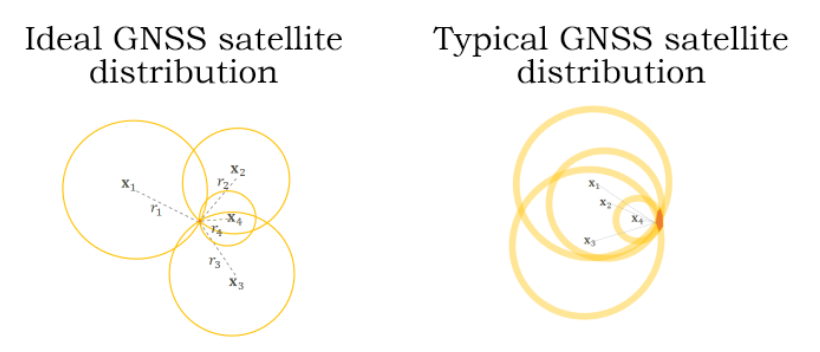
\includegraphics[width=0.7\textwidth]{img/wireless/satellite distibution.png}
          \caption{Distrubution of the satellites ideally and in reality}
          \label{fig:GNSS geometry}
        \end{figure}

        It can be proved that, under some conditions, this geometrical effect on the positioning 
        error can be measured.
        the standard deviation of the positioning error can be obtained as:
        \begin{equation}
          \sigma_{x} = \sqrt{\sigma^2_{x_u} + \sigma^2_{y_u} + \sigma^2_{z_u} + \sigma^2_{b_{ut}}}
          =\text{GDOP} \cdot \sigma_{\text{UERE}}
          \label{eq:GNSS PDOP}
        \end{equation}
        where GDOP is the \textbf{Geometric Dilution of Precision}:
        \begin{equation}
          \text{GDOP} = \sqrt{tr\{[H^TH]^{-1}\}}
          \label{eq:GNSS GDOP}
        \end{equation}
        and $\sigma_{\text{UERE}}$ is the standard deviation of the pseudorange error.\\
      \end{subsection}
    \end{section}

    \end{section}

    \begin{section}{GNSS threats}
      GNSS is not that robust by itself, in fact the main source of signal degradation are:
      \begin{itemize}
        \item \textbf{evil waveforms}
        \item \textbf{multipath}
        \item \textbf{radio frequency interference}
        \item \textbf{spoofing}
      \end{itemize}
      The robustness of GNSS signals derives from the \textbf{spread spectrum} nature of the 
      transmitted signal (Direct Sequence Spread Spectrum), exploited also for CDMA purposes.\\
      Despite the spread signal structure, navigation receivers are vulnerable to (strong) 
      interfering signals, that might prevent the correct signal processing.\\

      In fact, the typical signal to noise ration of a GNSS signal is around $-30dB$, which 
      means that on normal conditions the signal is buried in the noise.\\
      Fortunately, spread spectrum is robust to the presence of interfering signals, but we still
      have to revert the spreading to recover the original signal.\\
      The product with the PRN code spreads the power over a larger bandwidth, making the bandwidth
      of a signal $B_x \simeq 50 - 250\text{Hz}$ much larger($B_{SS} \simeq 2-8\text{MHz}$).\\
      If an interference signal of bandwidth $B_i$ affects the signal, only a portion of the power 
      will be actually received as “additional noise”, because the rest of the power will be
      spread over the whole bandwidth.\\

      For this reason, the despreading operation made at the receiver spreads the power of the 
      interfering signal over a wide bandwidth($B_{SS}$), making the interference power density
      much lower than the signal power density.\\

      \begin{figure}[h]
        \centering
        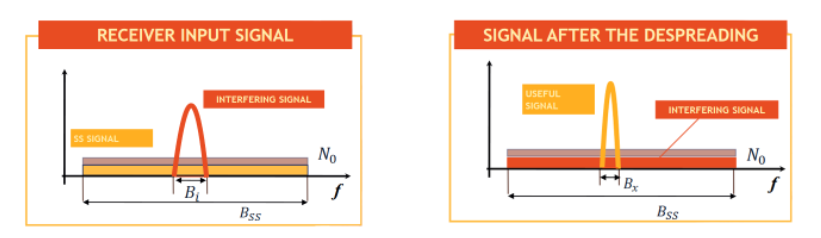
\includegraphics[width=0.9\textwidth]{img/wireless/signal despreading.png}
        \caption{Effect of despreading over a signal bandwidth}
        \label{fig:GNSS despreading}
      \end{figure}
      \begin{subsection}{Interference classification}
        Because of the bandwidth size, we are actually able to classify interference, according to 
        the spectral and time features with relation to the GNSS signal:
        \begin{itemize}
          \item \textbf{Narrowband Interference}: $B_i \ll B_{SS}$
          \item \textbf{Wideband Interference}: $B_i \simeq B_{SS}$
          \item \textbf{Continuous Wave Interference}: the interference is continuous in time
            over a single frequency band, $B_i \to 0$
          \item \textbf{Pulse Interference}: the interference is pulsed in time
        \end{itemize}

        We can also distinguish between \textbf{Out-of-band interference} and \textbf{In-band
        interference}.\\
        The first one is interference that is outside the GNSS band, while the second one is
        interference that is inside the GNSS band. This means that OOB interference should not 
        affect the GNSS signal, while IB interference can, buth both of them can be problematic.\\

        \begin{figure}[h]
          \centering
          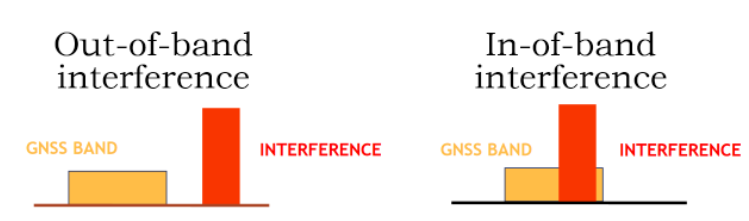
\includegraphics[width=0.7\textwidth]{img/wireless/in and out of band interference.png}
          \caption{Classification of interference}
          \label{fig:GNSS interference classification}
        \end{figure}

        A further distinction can be made between \textbf{Intentional Interference} and
        \textbf{Unintentional Interference}.\\
        The first one is interference that is intentionally generated to disrupt the GNSS signal,
        while the second one is interference that is generated by other devices, but that can still
        disrupt the GNSS signal, and is generally generated by OOB interference.\\
      \end{subsection}

      \begin{subsection}{Jamming}
        \begin{boxH}
          A \textbf{jammer} is a \textbf{device} that generates \textbf{interference} to disrupt the GNSS signal.\\
          Jamming objective is the denial of navigation service by masking the GNSS signal with
          noise.
        \end{boxH}

        Normally, signal radiation in the GNSSs bands is regulated by the ITU, and not legal.\\
        Those devices can be a severe threat for  liability-critical mass-market applications, 
        such as GNSS-based road tolling or fleet management.\\
        In general, Mass-market jammers usually aim at disturbing a wide band by 
        frequency-modulating a pure tone.\\

        Lets now try to understand the effect of jamming on the GNSS signal.\\
        In general, interference affect the receiver at different levels: at first we can observe 
        a spike in the noise level after the signal has been received, or we can observe a
        degradation of the signal quality.\\
        This means that we are able to understand if a signal is being jammed before the pseudorange
        is computed.\\

        The net effect is an error on the measured pseudorange $\rho$, and the effect depends on
        \begin{itemize}
          \item the receiver architecture(front-end filters, quantization bits, etc.)
          \item the structure of the GNSS signal(modulation, spreading, etc.)
        \end{itemize}
        Therefore detection and mitigation of interference can act at different stages of the 
        receiver itself:
        \begin{itemize}
          \item antenna shaping
          \item front-end filtering
          \item time domain blanking
          \item other transformed domains
        \end{itemize}

        \begin{figure}[h]
          \centering
          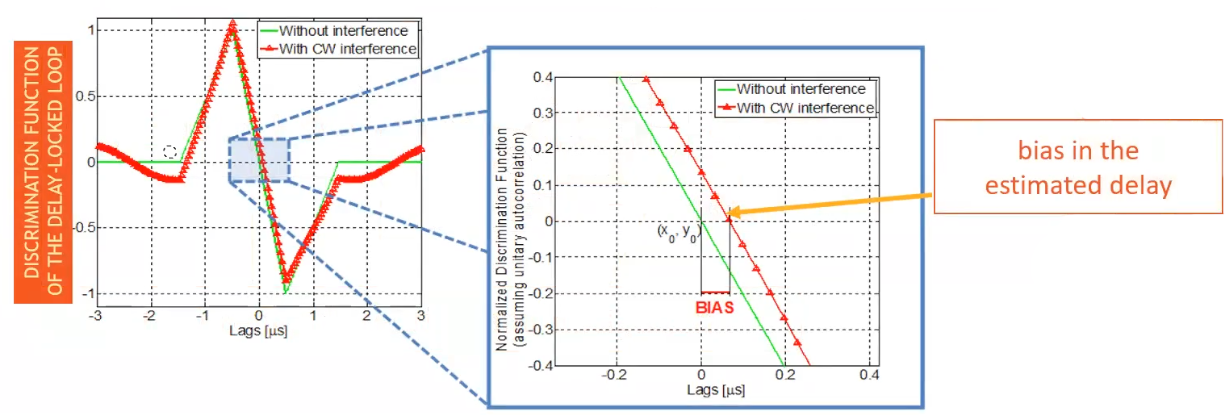
\includegraphics[width=0.7\textwidth]{img/wireless/jamming delay effect.png}
          \caption{Effect of jamming on the delay of a GNSS signal. The delay is increased by the
            jamming signal.}
          \label{fig:GNSS jamming effect}
        \end{figure}
        \begin{subsubsection}{Signal-to-Noise Ratio Monitoring}
          Aside from the spectrum, one other thing that can be monitored to detect jamming is the
          Signal-to-Noise Ratio(SNR).\\
          Strictly speaking, the interference is not noise, but from the user point of view it is
          indistinguishable from it. The net effect is that the SNR is affected by interference,
          contributing to the \textbf{noise variance}.\\

          Observing the SNR in some scenarios may allow to define a \textbf{statistical threshold}: 
          if the SNR is below a certain value, the signal may be jammed.\\

          Generally speaking, The only available output common to any GNSS receiver is the 
          carrier-to-noise-density ratio (C/N0) parameter, which is the ratio of the carrier power
          to the noise power spectral density, an estimated value closely related to SNR.\\
          The C/N0 is a good indicator of the signal quality, and it is used to detect jamming: in
          case of jamming, the C/N0 will decrease.\\
          \begin{figure}[h]
            \centering
            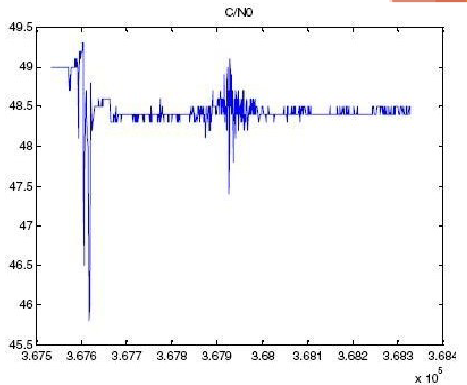
\includegraphics[width=0.3\textwidth]{img/wireless/c over n0.png}
            \caption{Example of a C/N0 measurements}
            \label{fig:GNSS CN0 monitoring}
          \end{figure}

        \end{subsubsection}
        \begin{subsubsection}{Spectral analysis}
          One of the most effective ways of detecting jamming is to perform a spectral analysis of the
          received signal.\\

          Figure \ref{fig:GNSS spectral analysis} shows the effect of interference on the spectrum
          of a GNSS signal.\\
          On the left is shown the effect of normal noise over the spectrum of the signal, while on
          the right is shown the effect of jamming.\\
          Is is evident when it is happening: you can clearly see it in the spectrum.\\

          \begin{figure}[h]
            \centering
            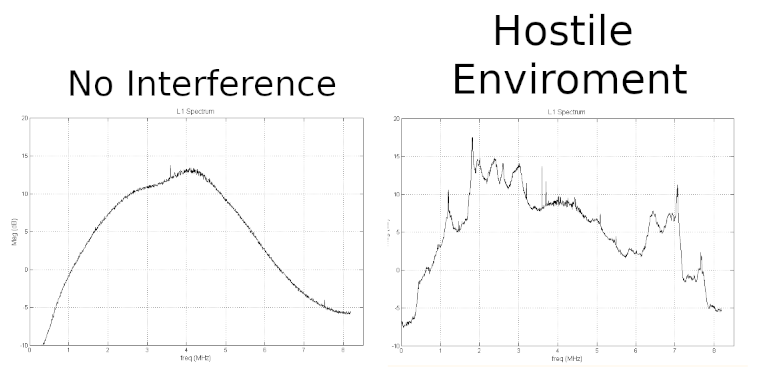
\includegraphics[width=0.7\textwidth]{img/wireless/spectrum effect.png}
            \caption{Effect of interference on the spectrum of a GNSS signal}
            \label{fig:GNSS spectral analysis}
          \end{figure}
        \end{subsubsection}
        \begin{subsubsection}{Automatic Gain Control Behavior}
          Another important detection strategy is to monitor the behavior of the Automatic Gain Control
          (AGC) of the receiver.\\

          The AGC is a system that automatically controls the gain of the receiver, in order to
          maintain the signal at a constant level, the optimal input range of the ADC(quantizer).\\
          \begin{figure}[h]
            \centering
            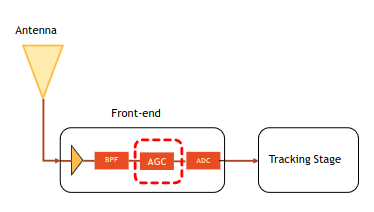
\includegraphics[width=0.4\textwidth]{img/wireless/AGC.png}
            \caption{Graphical representation of the AGC}
            \label{fig:AGC}
          \end{figure}
        It can be used to detect jamming, because the AGC will try to increase the increase the gain
        to maintain the signal at a constant level, but if the signal is jammed, the AGC will 
        decrease the gain because the signal is stronger.\\

        Because GNSS signals are weak, the AGC is usually set to a high gain, so if the AGC is
        decreasing the gain, it is a sign that the signal is being jammed.\\
        This is evident when looking at figure \ref{fig:AGC jamming}, which shows the gain level
        of the AGC over the time.\\
        n absence of interference the gain introduced by the AGC is constant over the time, or slowly
        changing, but in a hostile environment the average gain level is lower and the AGC
        gain is not constant.
        \begin{figure}[h]
          \centering
          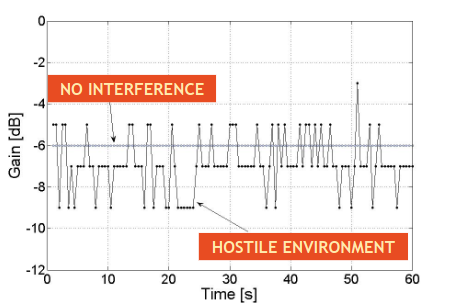
\includegraphics[width=0.6\textwidth]{img/wireless/AGC jamming.png}
          \caption{Effect of jamming on the AGC}
          \label{fig:AGC jamming}
        \end{figure}
        The AGC also have some kind of effect over the spectrum of the signal, decreasing the magnitude 
        of the spectrum over the intermediate frequencies(IF), and which is variable over time.\\
        

        \end{subsubsection}
        \begin{subsubsection}{Goodness-of-Fit Test}
          For interference detection purposes, the IF samples at the output of the ADC can be used 
          to build the test statistic and make the decision.\\
          The test performs the comparison of two Probability Density Functions (histograms),
          allowing the decision between two hypotheses. The PDFs are approximated by the histograms of
          the samples.
          
          If the thermal noise is dominating the samples distribution (nominal behavior), the 
          histogram should exhibit a \textbf{Gaussian shape}.
          On the other hand, In the case of the presence of an interference source, the histogram 
          will modify its regular shape, enabling the test to detect such a distortion.\\
          The bins needed for evaluating the discrete version of the PDF are directly arranged by 
          the signal quantization levels.

          \begin{boxH}
            In the \textbf{interference free} case the noise dominates the GNSS signal and the statistic of 
            samples is expected to be \textbf{Gaussian}.
          \end{boxH}

          \begin{figure}[h]
            \centering
            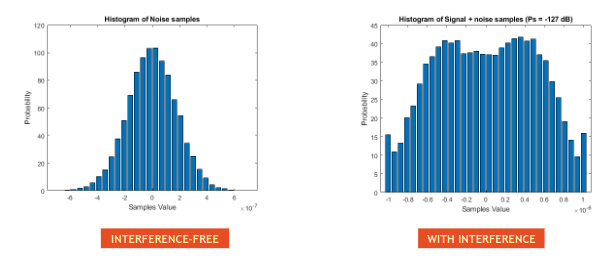
\includegraphics[width=0.8\textwidth]{img/wireless/good to fit test.png}
            \caption{Goodness-of-Fit test}
            \label{fig:GNSS goodness of fit}
          \end{figure}


        \end{subsubsection}

      \end{subsection}
      \begin{subsection}{Mitigation with domain techniques}
        For mitigation, we want to identify our interference precisely, in the time domain
        or frequency domain, depending on the nature of the interference.\\
        A continuous wave interference can be easily detected in the frequency domain, unlike in the 
        time domain, because the interference is occupying a single frequency band.\\

        To do so we can use a \textbf{notch filter}, which is a filter that removes a certain
        frequency band from the signal.\\

        In the time domain, we can understand when the interference is happening, and we can
        remove the interference by blanking the signal.\
      \end{subsection}
    \end{section}

    \begin{section}{Spoofing}
      \begin{boxH}
         Spoofing refers to the transmission of fraudulent GNSS-like signals, that force the
         victim receiver to compute erroneous positions
      \end{boxH}
      It is another big threat for GNSS. This kind of attack has been present in the military 
      field, but with the extensive use of GNSS it may threat several applications.\\

      Furthermore, while jamming is easily detectable, spoofing is not, because the signal is
      not masked by noise, but it is a signal that is very similar to the GNSS signal.\\
      For this reason, attacks can be very effective depending on the quality of the generated 
      signal.\\

      Denial of service is not the only possible attack, but by spoofing the signal, the attacker
      can also manipulate the position of the receiver, for example to fraud a tolling system.\\
      Such menaces also apply to safety-critical applications (e.g. Advanced Driver Assistance 
      Systems(ADAS), eCall).\\

      An ideal spoofer must be as much as possible consistent with the real signals, in fact it must
      \begin{itemize}
        \item Match the signals from expected visible satellite
        \item be synchronized with the GNSS time scale
        \item match the directing of arrival
        \item be realistic terms of power an Doppler effect(velocity)
      \end{itemize}
      Even a reply attack is enough to trick a receiver into a wrong position.\\

      \begin{subsection}{Meaconing}
        \begin{boxH}
          Meaconing is the reception and rebroadcasting of an entire block of RF spectrum 
          containing an ensemble of received GNSS signals, without distinction between different 
          satellite signals
        \end{boxH}
        Meaconing gets signals consistent with the real one and replay them with a variable delay
        so its difficult to counteract because, at the receiver level, the signals are consistent
        and must be \textbf{cross-checked}for detection.
        \begin{figure}[h]
          \centering
          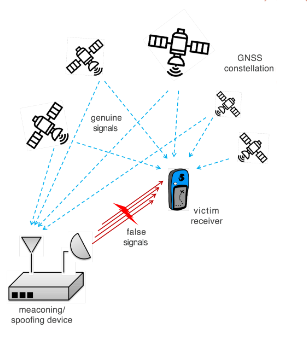
\includegraphics[width=0.4\textwidth]{img/wireless/meaconing.png}
          \caption{Meaconing attack}
          \label{fig:GNSS meaconing}
        \end{figure}

      \end{subsection}
    \end{section}


